\section{Introduction and Background} \label{sec:introduction}

The field of evolution, whether biological or digital, often involves the study of a large group of organisms and their genetic material.
A common question during these studies is how closely organisms are related to one another, and through phylogenetic analysis, ancestry trees can be built that outline the organisms' evolutionary history.
These trees have countless applications throughout the field, emphasizing the importance of accurate and efficient methods to reconstruct them.
However, with larger and larger datasets, latter becomes increasingly difficult, with some techniques proving infeasible at that scale.
Therefore, we present an algorithm that, in the scope of digital evolution, greatly improves the performance of phylogenetic reconstruction.

Phylogenetic analyses allow for characterizing and quantifying certain evolutionary processes, allowing researchers to make conclusions about the way a population evolved over time with varying degrees of accuracy depending on the method.
For example, fitness parameters such as growth rate, probability of survival, and so on \citep{genthon2023cell}.
Through large-scale analyses, patterns of evolutionary dynamics can be inferred, such as the effects of beneficial mutations on a population with varying levels of frequency \citep{levy2015quantitative}.
On the other hand, one may want to study the rate at which particular ancestor species split into many new species -- the speciation rate -- as well as the rate at which species die out -- the extinction rate.
By studying reconstructed phylogenies, both of these results can be determined \citep{stadler2013recovering}.

Phylogenetic analysis is also cruicial in the field of epidemiology, which becomes urgent in the face of pandemics such as COVID-19.
Through phylogenetic methods, we could determine which clade a particular strain came from, enabling the pinpointing of where and how a particular person was infected -- potentially leading to more efficient disease control \citep{wang2020role}.
In another case, researchers could use phylogenies to help identify ``super-spreaders'' -- diseases with a particularly high transmission rate -- that may cause massive outbreaks \citep{colijn2014phylogenetic}.

\subsection{Phylogenies \& Digital Evolution} \label{sec:introduction:digital}

Often, studying evolution through biological means is not as feasible, as laboratory experiements may take years, or even decades, to complete -- a canonical example being the long-term evolution experiment \citep{wiser2013long}.
Therefore, by simulating the behavior of a population, experiements can instead be done digitally, with simulations running in a fraction of the time.
These systems can model key characteristics of biological populations, such as variation, natural selection, facilitation, movement, predation, and more.
So, due to the nature of these simulations, conclusions about digital evolution can even be generalized to biological evolution \citep{pennock2007models, dolson2021digital}.

Since they use similar mechanisms as biological evolution, organisms that have evolved digitally can also be analysed through phylogenies.
One useful metric to determine if a population is likely to be successful is biodiversity, and digital populations are no exception.
In fact, by using phylogenetic diversity (as opposed to other methods such as phenotypic diversity), stronger conclusions could be made about a digital population's fitness \citep{hernandez2022phylogenetic}.

Digital evolution can also be performed in a manner that allows the testing of phylogenetic methods that are applicable to biological evolution.
The Aevol\_4b system, for instance, uses a genetic system corresponding to that of DNA, allowing any genetic information to be processed using methods directly from bioinformatics \citep{daudey2024aevol}.
Another system is SLiM which supports continuous-space modeling of multiple species at once \citep{haller2023slim}.

\subsection{Reconstructing Phylogenies} \label{sec:introduction:reconst}

When dealing with biological data, common methods for phylogenetic reconstruction include the analysis of DNA, looking at nucleotide changes between aligned sequences from different organisms. Note that this is a difficult problem, with popular algorithms being computationally expensive.
Common methods include distance-based methods, where a distance matrix between organisms is computed and processed with methods such as neighbor-joining \citep{saitou1987neighbor}; or character-based methods, such as maximum-parsimony \citep{sober1991reconstructing}, which seeks to minimize the number of evolutionary changes -- and maximum-likelihood \citep{felsenstein1981evolutionary}, which infers parameters about the tree that makes the given set of data most likely \citep{de2014phylogenetic}.

However, given the high controllability of digital simulations, many -- such as the aforementioned Aevol\_4b -- run with their own system of phylogenetic tracking, making (re)construction significantly easier when compared to traditional bioinformatics methods.
A simple example is perfect tracking: the idea that phylogenies can be tracked as the simulation runs. Many tools are designed specifically for this purpose \citep{dolson2024phylotrack}, while others simply incorporate bespoke implementations into their own software \citep{ofria2004avida}. However, large-scale distributed simulations, with limited memory and data integrity, are often unable to take advantage of perfect tracking.
When there are thousands -- if not millions -- of replications, perfect-tracking approaches become impractical due to \textbf{TODO}.
Therefore, they must instead opt for approximate tracking methods.

\subsection{Hereditary Stratigraphy} \label{sec:introduction:hstrat}

One method for approximate tracking of asexual organisms is hereditary stratigraphy, which acknowledges the fact that distributed systems may have limited memory per organism, and utilizes various algorithms to select what data to retain and what data to discard \citep{moreno2022hstrat}.
The end result is the genetic information of an organism being a series of rank-differentia pairs, where each rank represents a generation at which a datum was retained, and the differentia representing the datum itself.
However, the presence of missing information is a hurdle that a phylogenetic reconstruction algorithm must overcome, and may cause significant slowdowns using traditional algorithms.

\begin{figure*}

\centering
\begin{minipage}{0.75\textwidth}

\begin{minipage}{0.4\linewidth}
\centering
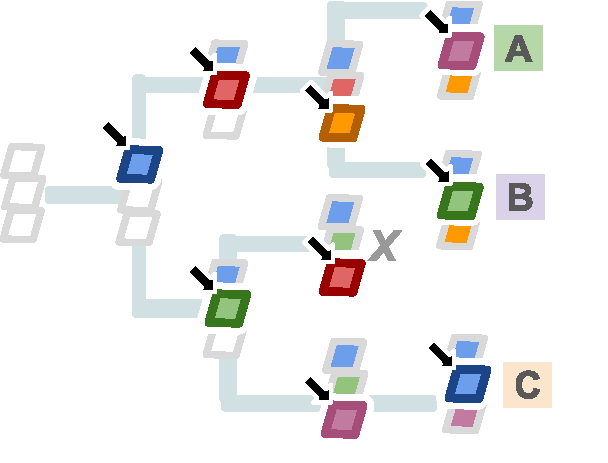
\includegraphics[height=1.5in]{img/hstratschematic-evolve}
\subcaption{evolve}
\end{minipage}%
\centering
\begin{minipage}{0.2\linewidth}
~~~
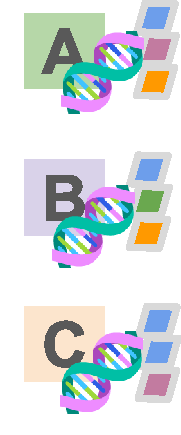
\includegraphics[height=1.5in]{img/hstratschematic-sample}
\subcaption{sample}
\end{minipage}%
\begin{minipage}{0.4\linewidth}
\centering
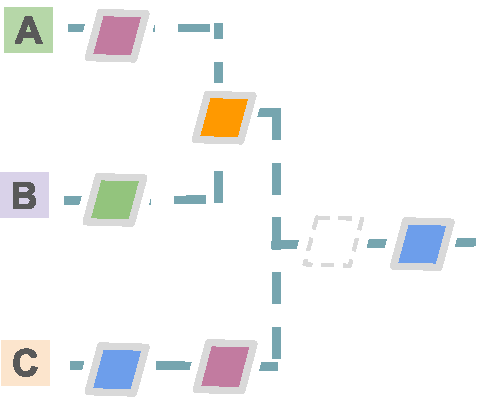
\includegraphics[height=1.5in]{img/hstratschematic-reconstruct}
\subcaption{reconstruct}
\end{minipage}
\end{minipage}%
\begin{minipage}{0.25\textwidth}
\caption{\textbf{TODO.}}
\label{fig:hstratschematic}
\end{minipage}

\end{figure*}

\textbf{TODO add more about hstrat}

\subsection{Problem Statement} \label{sec:introduction:problem}

The existing algorithm functions by treating the ordered rank-differentia pairs as strings (with potential missing information), where each differentia could represent a character at the rank-th position.
With this abstraction, we can essentially build a trie \citep{fredkin1960trie} from the organisms.

To begin, all organisms are sorted in ascending order by the number of generations elapsed; due to each organism using the same algorithm to determine which data to remove, if data at some rank is missing in one organism, it will be missing in all subsequent ones.
This list of organisms is then processed one at a time, going through each rank-differentia pair and determining whether to branch off the trie, continue along, or address missing information (see Algorithm~\ref{alg:old}).

If processing information corresponding to a rank $r$ that is larger than the rank $r'$ of a child $c$ of $n$, we know that the information at rank $r'$ must have been deleted in the original organism (otherwise, it would have been processed already).
To maximize reconstruction accuracy, we must deterrmine if the missing datum is child $c$'s differentia, that of another child also with rank $r'$, or by none of the children of $n$ (where we would branch off).
Essentially, when reaching missing information, we must infer that information, which we do by looking ahead on the tree. The naive  trie algorithm accomplished this by looking forwards and finding the path with the ``longest successive streak'' of matching differentia with the current organism \citep{moreno2024analysis}.
If there is no matching path, we simply branch off $n$ rather than through its children.

\begin{algorithm}[h]
    \caption{the existing algorithm for creating a phylogenetic tree through hereditary stratigraphy, using a naive trie-building approach}
    \label{alg:old}
    \begin{algorithmic}[1]
        \Require a list of organisms $O$ in ascending order by generations elapsed
        \Function{ReconstructTree}{$O$}
            \State $T \gets$ an empty tree
            \For {$o \in O$} 
                \State $\textsc{TreeInsert}(T, o)$
            \EndFor
            \State \Return $T$
        \EndFunction

        \Function{TreeInsert}{$T, o$}
            \State $n \gets$ root of $T$
            \For{each rank-differentia pair $(r, d) \in o$}
                \While{$r >$ the rank of $n$'s children}
                    \State $n \gets$ the child of $n$ most likely contain $o$
                \EndWhile
                \If{$\exists c \in \operatorname{children}(n) \text{ s.t.} \operatorname{differentia(c) = d}$}
                    \State $n \gets c$
                \Else 
                    \State create a new child $c'$ branching off $n$ 
                    \State $\operatorname{differentia}(c') \gets d$
                    \State $n \gets c'$
                \EndIf
            \EndFor
            \State insert information about $o$ as a child of $n$
        \EndFunction
    \end{algorithmic}
\end{algorithm}

However, despite being an accurate way of dealing with missing information, this approach suffers the cost of doing significant extra work each time.
In the worst case, there could be many matching paths to check, each with many matching differentiae.
In large-scale simulations, with limited differentia values (sometimes being represented with only one bit), this is a surprisingly common problem and significantly slows down the reconstruction process.
Additionally, these searches would need to happen for each organism, regardless of whether or not a similar search was already done.
Therefore, we present an improved algorithm that consolidates this extra work into a single step, never needing to be repeated.
